\documentclass[table, 12pt]{article}
\usepackage[T1]{fontenc}
\usepackage[utf8]{inputenc}
\usepackage[english]{babel}
\usepackage{graphicx}
\usepackage{titlesec}
\usepackage{hyperref}
\usepackage[table]{xcolor}
\usepackage{float}

\hyphenation{Te-lan-ga-na}
\hyphenation{an-a-lys-ing}
\titleformat{\paragraph}
{\normalfont\normalsize\bfseries}{\theparagraph}{1em}{}
\titlespacing*{\paragraph}
{0pt}{3.25ex plus 1ex minus .2ex}{1.5ex plus .2ex}


\begin{document}
\begin{titlepage}
    \centering
    {\scshape\large AY 2021/2022 \par}
    \vfill
    
\includegraphics[width=100pt]{assets/logo-polimi-new}\par\vspace{1cm}
    {\scshape\LARGE Politecnico di Milano \par}
    \vspace{1.5cm}
    {\huge\bfseries RASD\@: Requirement Analysis
        and Specification Document \par}
    \vspace{2cm}
    {\Large {Ottavia Belotti\quad Alessio Braccini\quad Riccardo Izzo}\par}
    \vfill
    {\large Professor\par
        Elisabetta \textsc{Di Nitto}}
    \vfill
    {\large \textbf{Version 1.0}\\ \today \par}
\end{titlepage}

\hypersetup{%
    pdfborder = {0 0 0}
}

\thispagestyle{plain}
\pagenumbering{gobble}
\mbox{}
\newpage
\pagenumbering{roman}
\tableofcontents
\newpage
\pagenumbering{arabic}

\section{Introduction}
\emph{Data-dRiven PrEdictive FArMing}, also known as \emph{DREAM}, is a project presented by UNDP India and Healthsites initiative, promoted by Telangana's government.
The aim of the project is to enhance the farm system and the entire food supply chain with an IT supporting application. 
This arises from modern challenges like climate change and the foreseen population growth that have underlined the critical issues of the modern system making necessary a complete overhaul.


\subsection{Purpose} %goals of the project
\emph{DREAM} aims to support work categories involved into the farming industry by providing them relevant and up-to-date data about the farm activity's performance. 
The main stakeholders are: Telangana's policy makers, farmers and agronomists.
The goal is to develop a data-driven application with the help of IT partners.
Telangana's state already collect important data concerning wheather forecast, these data are publicly available with a live rainfall map on the official government website.
Other data can be collected through humidity sensors deployed all over the territory and through the water irrigation system.

Agriculture has a main role in India's economy, more than half of the population depends on it and about a fifth is below the poverty line.
Furthermore, as a significant increment in population is expected for 2050 (\emph{UN}'s esteem), food demand is going to significantly increase.
Telangana needs an efficient application to increase the general productivity of the farm system.

The user base is expected to be the entire population of Telangana, starting with those who works in the agricolture sector up to normal citizens.

\subsection{Scope} %analysis of the world and shared phenomena
%ADD: basic service and advanced functionalities
\subsubsection*{Phenomena controlled by the Machine}
\rowcolors{2}{gray!50}{}
\begin{tabular}{|c|c|c|}
    \hline
    \textbf{ID} & \textbf{Phenomenom} & \textbf{Shared} \\\hline\hline
    M1 & Check username and password & No \\\hline
    M2 & Analysis of best practices & No\\\hline
    M3 & Analysis of weather data & No \\\hline
    M4 & Visualize data concerning weather, land, performance & Yes\\\hline
    \hline
\end{tabular}

\subsubsection*{Phenomena controlled by the World}
\begin{center}
    \rowcolors{2}{gray!50}{}
    \begin{tabular}{|c|c|c|}
        \hline
        \textbf{ID} & \textbf{Phenomenom} & \textbf{Shared} \\\hline\hline
        W1 & User login & Yes\\\hline
        W2 & User share best practice & Yes\\\hline
        W3 & User ask for help on forum & Yes\\\hline
        W4 & Collect land data from sensor & Yes\\\hline
        W5 & User create topic in forum & Yes\\\hline 
        W6 & User insert post & Yes\\\hline
        W7 & User reply to a post & Yes \\\hline
        W8 & User update daily plan & Yes\\\hline
        W9 & User check weather forcast & Yes\\\hline
        \hline
    \end{tabular}
\end{center}

\subsubsection{Goals}
\underline{Telangana's policy makers}
\begin{enumerate}
    \item \textbf{Identification of well-performing farmers}\\
    Main goal of the policy makers is to identify farmers that are resilient to meteorological adverse events.
    This can be done comparing the productivity ratio defined as the produced amount per product in adverse condition over the amount in standard conditions.
    This farmers will receive special incentives and will be asked to help other farmers 
    with useful practices.
    \item \textbf{Identification of bad-performing farmers}\\
    Identify farmers that are performing bad using the productivity ratio, they are the ones that need to be helped 
    by the well-performing farmers.
    \item \textbf{Visualize the results of steering initiatives}\\
    Visualize and evaluate the results produced by the steering initiatives from agronomists and good farmers.
\end{enumerate}

\underline{Farmers}
\begin{enumerate}
    \item \textbf{Visualize data}\\
    Visualize important data like weather forecast and personalized suggestion about specific crops or fertilizers.
    All data are based on location and type of production.
    \item \textbf{Insert data}\\
    Insert data about their production, report every type of problems.
    \item \textbf{Request for help/suggestion}\\
    Farmers can request help with a text message that will be sent directly to the agronomists responsible of the area.
    \item \textbf{Create discussion forums}\\
    Create forums to discuss with the other farmers.
    In this section the creator can choose the name of the forum and invite all the desirable partecipants.
\end{enumerate}

\underline{Agronomists}
\begin{enumerate}
    \item \textbf{Insert area}\\
    Insert the area of responsibility for the agronomist.
    \item \textbf{Receive request for help/suggestion}\\
    Here the agronomist can manage all the incoming request for help or suggestion.
    This can be done with a specific section where the agronomist can visualize the message and answer it.
    \item \textbf{Visualize area stats}\\
    Visualize data about whether forecast or a list of best-performing farmers.
    The list of best-performing farmers is based on the productivity over a selected period of time.
    \item \textbf{Visualize and update daily plan}\\
    The daily plan consists in a list of farms to be visited during the day.
    Every farm must be visited at least twice a year with particular attention to the under-performing ones that 
    should be visited more often.
    \item \textbf{Confirm the daily plan}\\
    Confirm the daily plan at the end of the day or update it in case of deviations.
\end{enumerate}

\subsection{Definitions, acronyms, abbreviations}
\subsubsection*{Definitions}
\subsubsection*{Acronyms}
\begin{itemize}
    \item \textbf{RASD}: Requirement Analysis and Specification Document
    \item \textbf{DREAM}: \emph{Data-driven predictive farming} project
    \item \textbf{Telangana}: Indian state promoting the \emph{DREAM} project
\end{itemize}
\subsection{Revision history}
\subsection{Reference documents}
\begin{itemize}
    \item Specification document: "Assignment RDD AY 2021-2022"
    \item Alloy documentation: https://alloytools.org/documentation.html
    \item UML documentation: https://www.uml-diagrams.org/
    \item BPMN documentation: https://www.bpmn.org/
    \item Paper: "The World and the Machine" by M. Jackson and P. Zave
\end{itemize}

\subsection{Document structure}
\begin{itemize}
    \item \textbf{Section 1} gives an introduction about the problem to tackle and about which functionalities will be implemented in the final product in order to solve it.
    \item \textbf{Section 2} contains the overall description of the whole project, presenting it in a more formal way through class diagrams which will contain the backbone blocks that will build the final application. Furthermore, there will be presented the so-called \emph{actors} who are the ones that will use the application, the expected functionalities and the domain assumptions taken in consideration throughout the whole project, from the specification phase to the actual developing phase.
    \item \textbf{Section 3} delves deeply into the technical aspects of the topics presented in \emph{Section 2}, in order to be more useful for the development, by providing a standard interfaces' system \textit{a priori} to  stick to during the project implementation. It will show functional and non-functional requirements. The former will be presented through some use-cases and scenarios as meaningful examples; while the latter will be disclosed by analysing performance, design and software system features that the project will have.
    \item \textbf{Section 4} presents the Alloy code briefly explainig the purpose of it in modeling the given problem.
\end{itemize}

\section{Overall Description}
\subsection{Product perspective}
DREAM is a system that offers the functionalities described in the \textit{Product Functions (\ref{product_functions})} section.
It manages to use some external interfaces, for more details refers to the \textit{Software Interfaces (\ref{software_interfaces})} section.
We can see below an high-level class diagram that shows the basic structure of the system.
\subsubsection{Class diagram}
A UML class diagram that describes the main entities in the system.
Three types of actors can access the system: farmers, policy makers and agronomists.
During sign up they all create a user account with basic informations such as username, password and email.
At this point users are requested to insert other informations based on their type of account.
For example, to complete the registration, farmers need to specify the address of their farm and agronomists must declare their area of responsability.
The system provides several functionalities, one of this is the forum.
When the farmers select the forum section they basically access the topics that are characterized by a list of messages where the sender is specified. 
The agronomists can confirm and update a daily plan.
This is composed by the current date, the list of farms visited and a status flag that indicates whether the plan has already been confimed or not.
Moreover they have access to the list of farmers currently under their area of responsability.
Finally there are various type of data that can be visualized and analyzed by the users, which ones to display dependes on the type of account.
There are four types of data:
\begin{itemize}
    \item Sensor data\\
    Acquired by the sensors distributed all over the territory, characterized by a value that is the humidity of soil.
    \item Weather forecast data\\
    Meteorological short-term and long-term forecast acquired by the Telangana's government and displayed on their official website.
    The data to display to the user are temperature, rainfall, wind and humidity.
    \item Water irrigation data\\
    Acquired by the water irrigation system installed in the farm, the only significant value is the amount of water.
    \item Production data\\
    Provided by the farmers, this type of data is displayed as a table that map the type of product to the amount produced.
\end{itemize}
\begin{center}
    \begin{figure}[!h]
        \hspace{-110px}
        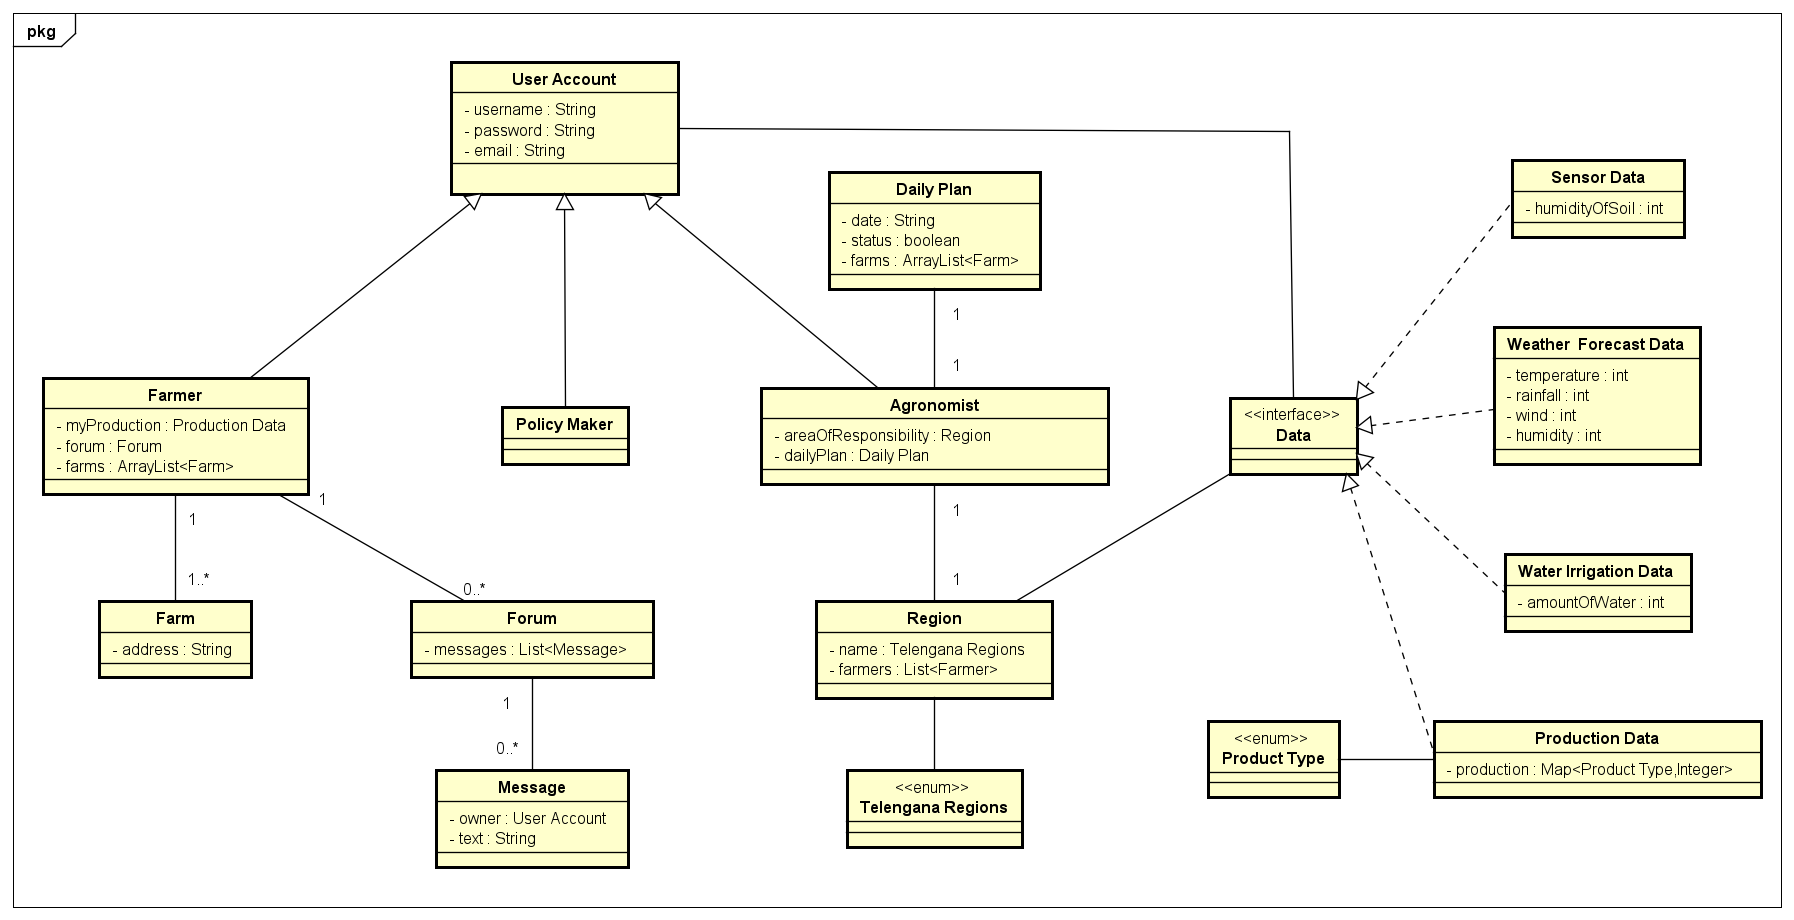
\includegraphics[scale=0.45]{assets/UML/UML.png}
        \caption{High-level UML}
        \label{fig: UML}
    \end{figure}
\end{center}
\newpage
\subsection{Product functions}
\label{product_functions}
\subsubsection{Sign-up and shared functions}
\begin{itemize}
    \item \textbf{Sign-up:} let the user sign-up thorugh an email and a password, creating a profile tailored for the user's job. Specify the area in which they live and what type of cultivation they manage.
    \begin{center}
        \begin{figure}[!h]
            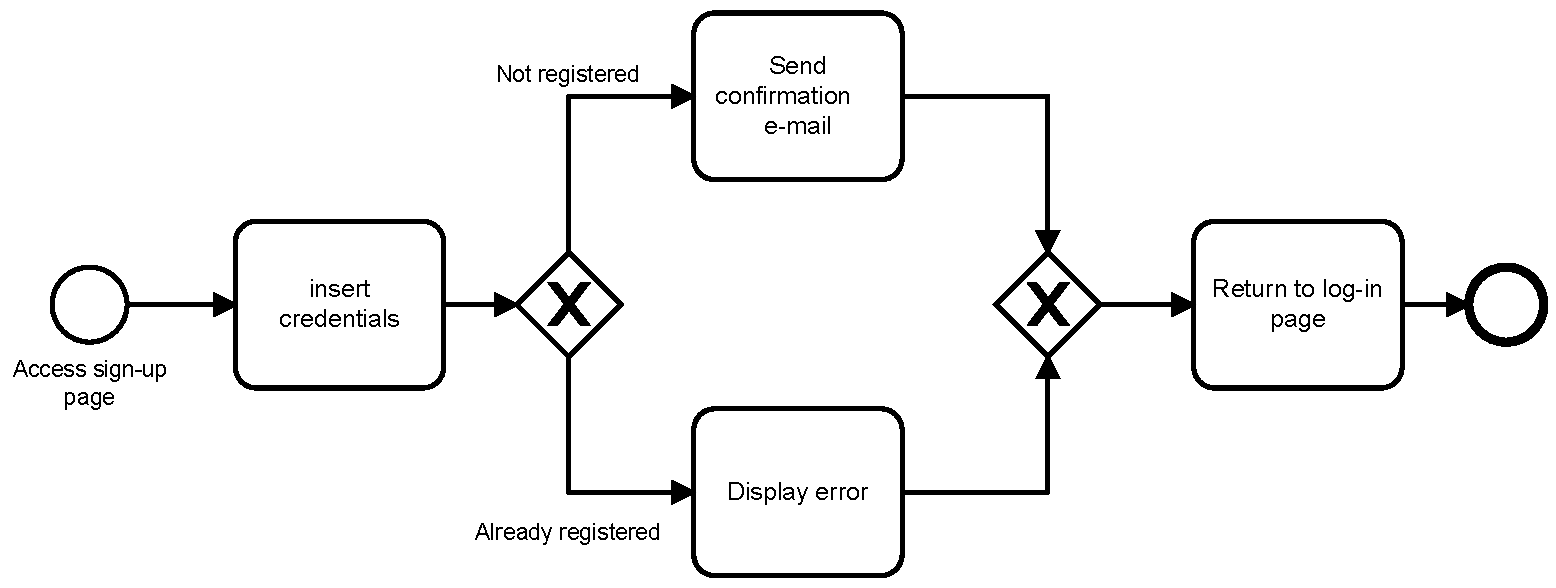
\includegraphics[width=\textwidth]{assets/BPMN/SignUpBpmn}
            \caption{Sign Up BPMN}
            \label{fig: singup}
        \end{figure}
    \end{center}
\end{itemize}
\subsubsection{Policy makers functions}
\begin{itemize}                                 
    \item \textbf{Visualize relevant data and initiative: }let the policy makers know a variety of different data like the performances of the farmers by grouping them in a rank to know who are the farmers that are performing well and who are the worst one based on informations insert by them.
    Policy makers can also visualize the steering iniziative presented by the agronomist in a specific subsection of their system.
\end{itemize}
\subsubsection{Farmers functions}
\begin{itemize}
    \item \textbf{Profile edit: }allow the farmers change their profile in order to upgrade information like: 
    \begin{itemize}
        \item[] Area: allow to change the area where farmers have their plantation;
        \item[] Plant type: allow to change the type of plant;
        \item[] Username and password: allow to change their username and password.
    \end{itemize}
    \begin{center}
        \begin{figure}[!h]
            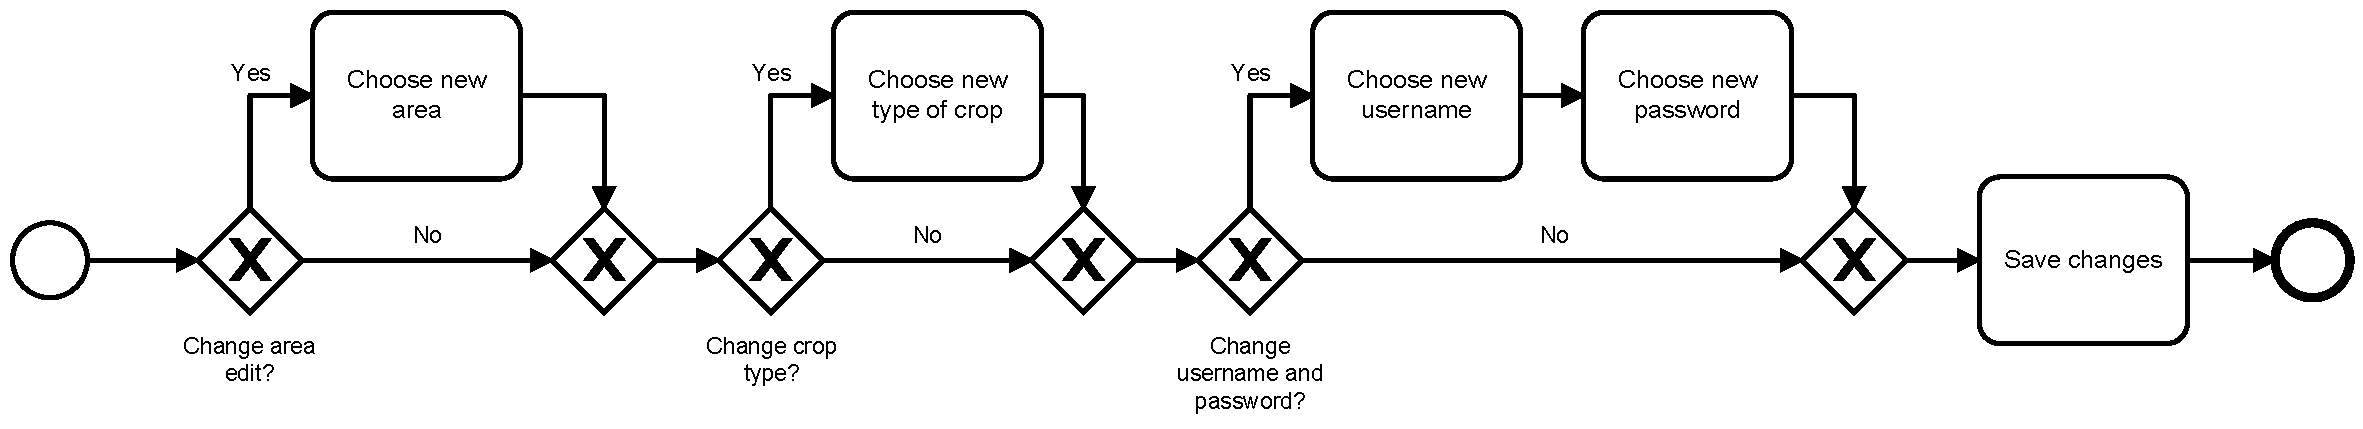
\includegraphics[width=\textwidth]{assets/BPMN/ProfileEditBpmn}
            \caption{Profile edit BPMN}
            \label{fig: profileedit}
        \end{figure}
    \end{center}
    \item \textbf{Manipulation of informations: }allow farmers to visualize every kind of their interest like the wheather forecast for the day or for the next few days or some suggestions about own crops and specific fertilizers.
    \item \textbf{Send message: }allow farmers to send messages to the agronomist.
    \item \textbf{Usage of the forum: }allow farmers to create a new topic or reply to a message in the dedicated forum.
    \item \begin{center}
        \begin{figure}[!h]
            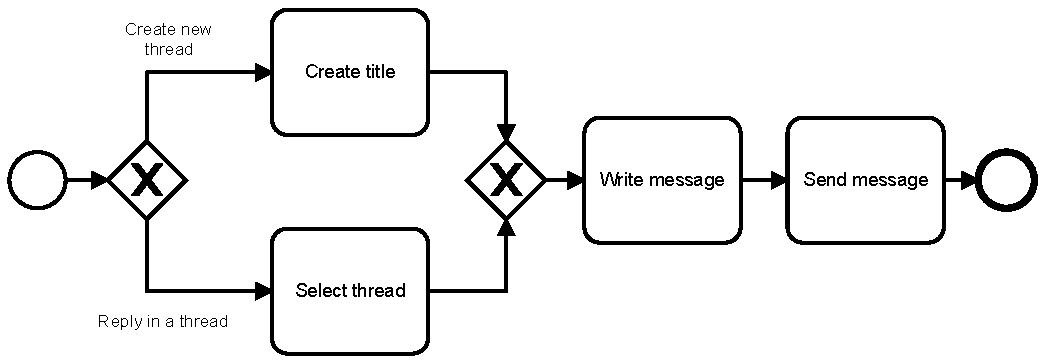
\includegraphics[width=\textwidth]{assets/BPMN/ForumBpmn}
            \caption{Forum BPMN}
            \label{fig: forum}
        \end{figure}
    \end{center}
\end{itemize}
\subsubsection{Agronomists functions}
\begin{itemize}
    \item \textbf{Area functions: }allow the agronomist to insert their responsability area and visualize the correspondant data like wheather forecast or the rank of the farmers.
    \item \textbf{Manage farmers requests: }farmers can send help or suggestion request to whom agronomist have to reply.
    \item \textbf{Manage daily plan: }allow the agronomist to make their daily plan by registring the incoming visits to the farmers. At the end of the day a farmers must confirm if they were able to complete the plan or specify the deviations occurred during the day.   
    \begin{center}
        \begin{figure}[!h]
            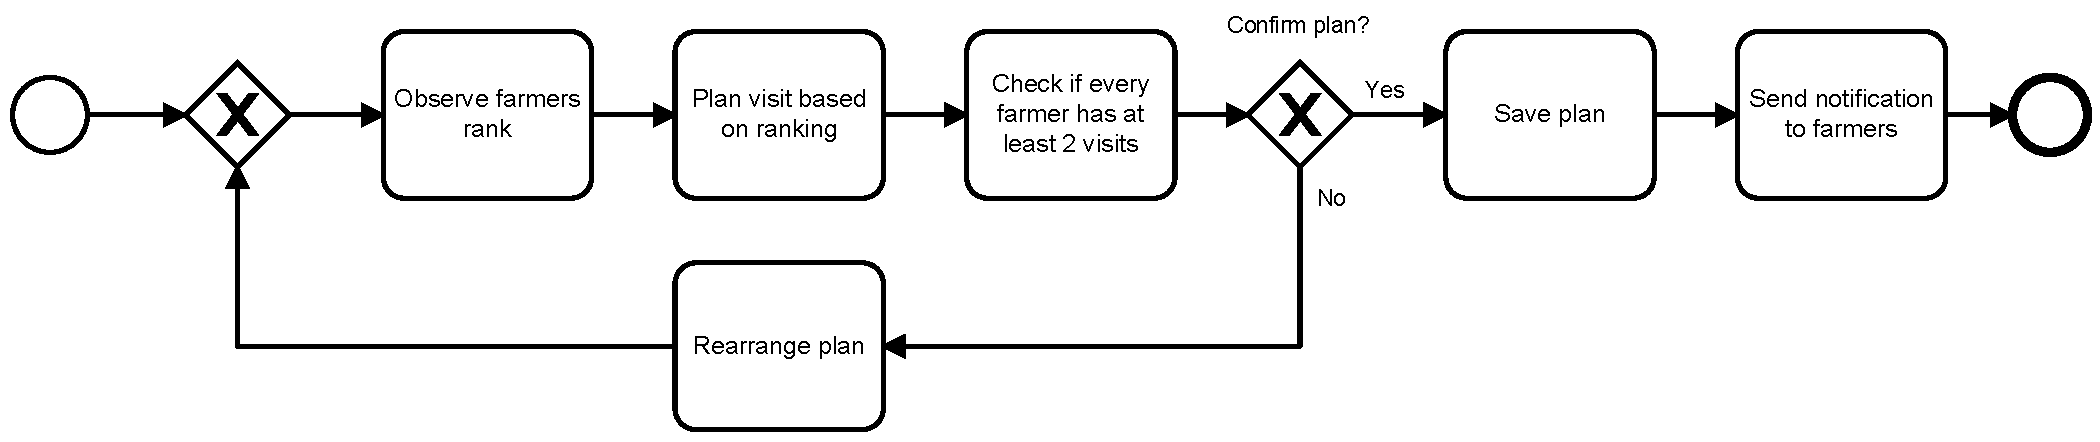
\includegraphics[width=\textwidth]{assets/BPMN/DailyPlanBpmn}
            \caption{Daily plan BPMN}
            \label{fig: dailyplan}
        \end{figure}
    \end{center}
\end{itemize}

\subsection{User characteristics}
The application has been thought for the three different user categories that follows:
\begin{itemize}
    \item \textbf{Policy makers} are government's employees that are in charge of analysing the general agricolture trends among all the districts in Telangana, then promote based state-wide policies to better the whole food system. Their main goal is not only to secure the current provision, but also to identify now the best practices that will lead to a flourishing food production in the future. By doing so, the plan is to grow more resiliant and profitable crops and prepare the lands to face future menaces, for instance the climate that is getting more hostile or the foreseen increment of the food demand. As a consequence, they want to be notified about the best performing farmers in order to contact them and get more insight from them about their procedures, with the aim to acquire best practises to be shared and applied on a larger scale. At the same time, they need to know who, on the other hand, is performing particularly badly, so that they can be given the help they need to better their results, since obtaining the foresaid goal requires the structure to run smoothly in all its parts. 
    Policy makers also need a feedback system that let them be aware of the true impact \textit{a posteriori} of the initiatives carried out by the agronomists in collaboration with the knowledge and practice of the best farmers.
    \item \textbf{Farmers} are interested in functionalities that will help with their day-to-day life at work, so they would like to receive in one place all the information about the weather to plan before hand the work day and useful data, like suggestions and news about the specific crop they cultivate, if some crop's illness is spreading in their area and how to treat it, which fertilizers boost the plant's production, etc. Moreover, they should insert data about their own production and ask for help to a regional agronomist through the app if it's needed. Being part of a larger community of people that share the same purpose (such as being more productive) brings more knowledge in general, so it's easier for the farmers to get in touch with their collegues that grow the same crops and might have faced the same challenges they do through the in-app forum. The feature allows them to enlarge their pool of acquaintances and brings them together online, even though they might be kilometers away from each other.
    \item \textbf{Agronomists} are the experts in the agricolture field, so the main function needed for them is the possibility of helping out the farmers that reach out to them. Each agronomist is in charge of a specific geographical area in Telangana, in order to be efficiently present on the territory in a fair and useful way according to the actual helping demand. In fact, they visit each farm spread among their area at least twice a year. That said, agronomists would like some functionalities that help them planning out their trips on the field in an simple yet flexible way. Furthermore, they would like to be notified of the farms' performace, especially the ones scoring poor results in order to plan their visits more often for those, depending on the problem their facing. Nonetheless, in order to make a complete and axhaustive report about the area productivity for the central government, they are also interested into acknowledging the top performing farms. %wheather forcast? go deeper in explaining daily plan funct?
\end{itemize}
\subsection{Assumptions, dependencies and constraints}
\begin{itemize}
    \item D1: Agronomists actually stick to the scheduled daily plan
    \item D2: Agronomists correct their schedule at the end of the day if deviations occur
    \item D3: Each user registers according to their role and always feeds correct information to the app
    \item D4: The internet connection works properly
    \item D5: The sensors measuring humidity level of the soil work properly
    \item D6: Weather forecasts are accurate up to a 80\% for the short-term and up to 60\% on the long-term
    \item D7: Water irrigation system send the information accurately, with an error of at most 1\%
    \item D8: Agronomists always replay to farmers requests of help
    \item D9: Farmers periodically insert data about their crop status and resulting production
\end{itemize}

\section{Specific Requirements}

\subsection{External Interface Requirements}

\subsubsection{User Interfaces}
The system should interface with users through devices which must be connected to the Internet.
Everyone that needs to use this service would connect to it through a web broswer from an existing domain, for example: dream.com.
It must be easy to use as it will have to be used from different kind of people, sometimes with a not great affinity with technologies.

\subsubsection{Hardware Interfaces}
The system "as it is" does not provide specific hardware equipment in order to access to web site. To use all functionalities it's required to have an IT devices connected to the internet, eventually a user can decide to use GPS to insert his own location and only proper devices with GPS equipment can do this. 

Soil data, obtained from sensors, are collect by someone else and will be added by the policy makers, also this not requires any special kind of hardware.

\subsubsection{Software Interfaces}
\label{software_interfaces}
In order to use the system it's required the use of a web broswer, on that will run the application.

System will also use some important interfaces in order to accomplish its functionalities.

First is an external API to access maps which will use the position acquired by the user settings to return an interactive map with a marker on that exact position.

Second API service used is the one of the DBMS system which will be adopted in order to query the internal database.

Another API will be use to access the external database containing data reguarding the sensor data and the other external data that the system need.

\subsubsection{Communication Interfaces}
Internet connection is mandatory in order to access to every formation that the system will display.
Users that want full functionalities have to have a GPS system on their device in order to guarantee a certain level of precision in the localization phase.

\subsection{Functional Requirements}

\subsubsection{List of Requirements}

\subsubsection{Mapping}

\subsubsection{Use Cases}
\setcounter{secnumdepth}{4}

    \paragraph{Use Cases Diagram}


    \paragraph{Use Cases Description}
    
        \begin{itemize}
            \item \textbf {Shared Use Cases}

            
            \begin{table}[H]
                \item[] \textbf{Sign Up}
                \item[] 
                \centering
                \begin{tabular}{c m{.70\textwidth}}
                    \hline
                    \textbf{Use Case} & Sign Up\\ 
                    \textbf{Actor} & Policy Maker, Farmer, Agronomist\\ \hline
                    \textbf{Entry condition} & User want to register in the system\\  \hline
                    \textbf{Flow of events} & \begin{enumerate}
                                                \item User press the sign up button
                                                \item User select its username, password and role
                                            \end{enumerate}\\ \hline
                    \textbf{Exit condition} & The system shows a confirmation message to the user \\ \hline
                    \textbf{Exceptions} &  \begin{enumerate}
                        \item If the user insert an already taken username
                        \item If the user press the cancel button
                        \item Internet connection isn't working
                    \end{enumerate}\\ \hline                    
                \end{tabular}
            \end{table}

            
            \begin{table}[H]
                \item[] \textbf{Log In}
                \item[]  
                \centering
                \begin{tabular}{c m{.70\textwidth}}
                    \hline
                    \textbf{Use Case} & Log In\\ \hline
                    \textbf{Actor} & Policy Maker, Farmer, Agronomist\\ \hline
                    \textbf{Entry condition} & User want to log in the system\\  \hline
                    \textbf{Flow of events} & \begin{enumerate}
                                                \item User put its own username and password
                                            \end{enumerate}\\ \hline
                    \textbf{Exit condition} & The system correctly log in the system\\ \hline
                    \textbf{Exceptions} &  \begin{enumerate}
                        \item If the user insert a wrong username and password
                        \item Internet connection isn't working
                    \end{enumerate}\\ \hline                    
                \end{tabular}
            \end{table}

            \item \textbf{Policy Makers}
            
            
            \begin{table}[H]
                \item[] \textbf{View Initiative Report}
                \item[] 
                \centering
                \begin{tabular}{c m{.70\textwidth}}
                    \hline
                    \textbf{Use Case} & View Initiative Report\\ \hline
                    \textbf{Actor} & Policy Maker\\ \hline
                    \textbf{Entry condition} & User wants to check the Steering Initiative proposed by agronomists\\  \hline
                    \textbf{Flow of events} & \begin{enumerate}
                                                \item User press the "View Initiative Reports" button
                                                \item System send to the user the steering initiative insert by the agronomist
                                            \end{enumerate}\\ \hline
                    \textbf{Exit condition} & User press the back button \\ \hline
                    \textbf{Exceptions} &  \\ \hline                    
                \end{tabular}
            \end{table}
                
            
            \begin{table}[H]
                \item[] \textbf{Check Soil Humidity Data}
                \item[] 
                \centering
                \begin{tabular}{c m{.70\textwidth}}
                    \hline
                    \textbf{Use Case} & Check Soil Humidity Data\\ \hline
                    \textbf{Actor} & Policy Maker \\ \hline
                    \textbf{Entry condition} & User wants to check the soil humidity data\\  \hline
                    \textbf{Flow of events} & \begin{enumerate}
                                                \item User press the "Check Sensors Data" button
                                                \item User press the soil humidity data button
                                                \item System retrive soil humidity data and send them back to the user
                                                \item System display the data
                                            \end{enumerate}\\ \hline
                    \textbf{Exit condition} & User press the "Home" button\\ \hline
                    \textbf{Exceptions} &  \\ \hline                   
                \end{tabular}
            \end{table}

            
            \begin{table}[H]
                \item[] \textbf{Check Water Irrigation Data}
                \item[] 
                \centering
                \begin{tabular}{c m{.70\textwidth}}
                    \hline
                    \textbf{Use Case} & Check Water Irrigation Data\\ \hline
                    \textbf{Actor} & Policy Maker \\ \hline
                    \textbf{Entry condition} & User wants to check the water irrigation data\\  \hline
                    \textbf{Flow of events} & \begin{enumerate}
                                                \item User press the "Check Sensors Data" button
                                                \item User press the water irrigation button
                                                \item System retrive water irrigation data and send them back to the user 
                                                \item System display the data
                                            \end{enumerate}\\ \hline
                    \textbf{Exit condition} & User press the "Home" button\\ \hline
                    \textbf{Exceptions} &  \\ \hline                   
                \end{tabular}
            \end{table}

           
            \begin{table}[H]
                \item[] \textbf{View Farmers Ranking}
                \item[] 
                \centering
                \begin{tabular}{c m{.70\textwidth}}
                    \hline
                    \textbf{Use Case} & View Farmers Ranking\\ \hline
                    \textbf{Actor} & Policy Maker\\ \hline
                    \textbf{Entry condition} & User wants to see the farmers ranking\\  \hline
                    \textbf{Flow of events} & \begin{enumerate}
                                                \item User press the best or the worst performing ranking
                                                \item System retrive data on farmers ranking
                                                \item System show ranking data 
                                            \end{enumerate}\\ \hline
                    \textbf{Exit condition} & User press the "Back" button\\ \hline
                    \textbf{Exceptions} &  \\ \hline                    
                \end{tabular}
            \end{table}

            
            \begin{table}[H]
                \item[] \textbf{View Specific Farmer Informations (View Farmers Ranking)}
                \item[] 
                \centering
                \begin{tabular}{c m{.70\textwidth}}
                    \hline
                    \textbf{Use Case} & View Specific Farmer Informations (View Farmers Ranking)\\ \hline
                    \textbf{Actor} & Policy Maker\\ \hline
                    \textbf{Entry condition} & User wants to see the specific informations of a farmer\\  \hline
                    \textbf{Flow of events} & \begin{enumerate}
                                                \item First three events are the same of the "View Farmers Ranking" use case 
                                                \item User press on a farmer name
                                                \item System retrive farmer data 
                                                \item System display farmer data
                                            \end{enumerate}\\ \hline
                    \textbf{Exit condition} & User press "Back" button\\ \hline
                    \textbf{Exceptions} &  \\ \hline                    
                \end{tabular}
            \end{table}
            
            \item \textbf {Farmers}
            
            
            \begin{table}[H]
                \item[] \textbf{Profiel Edit}
                \item[] 
                \centering
                \begin{tabular}{c m{.70\textwidth}}
                    \hline
                    \textbf{Use Case} & Profile Edit\\ \hline
                    \textbf{Actor} & Farmers\\ \hline
                    \textbf{Entry condition} & User wants to modify or update its profile\\  \hline
                    \textbf{Flow of events} & \begin{enumerate}
                                                \item User press the "Settings" button on its home page
                                                \item User modify the interest data (username, password, crop type or area)
                                                \item User press "Confirm" button
                                            \end{enumerate}\\ \hline
                    \textbf{Exit condition} & User receive a confirmation message\\ \hline
                    \textbf{Exceptions} &  \begin{enumerate}
                        \item User choose an already taken username
                        \item User choose the old password
                    \end{enumerate}\\ \hline                    
                \end{tabular}
            \end{table}

            
            \begin{table}[H]
                \item[] \textbf{Insert Production Data}
                \item[] 
                \centering
                \begin{tabular}{c m{.70\textwidth}}
                    \hline
                    \textbf{Use Case} & Insert Production Data\\ \hline
                    \textbf{Actor} & Farmers\\ \hline
                    \textbf{Entry condition} & User wants to insert the production data\\  \hline
                    \textbf{Flow of events} & \begin{enumerate}
                                                \item User press the "Insert Production Data" button
                                                \item User insert data reguarding its coultivation performance
                                                \item User press "Confirm" button
                                                \item System collect and analiyze data
                                            \end{enumerate}\\ \hline
                    \textbf{Exit condition} & User receive a confirmation message\\ \hline
                    \textbf{Exceptions} &  \begin{enumerate}
                        \item User insert data in a wrong manner
                        \item User press "Back" button
                    \end{enumerate}\\ \hline                    
                \end{tabular}
            \end{table}
            
            
            \begin{table}[H]
                \item[] \textbf{Check News}
                \item[] 
                \centering
                \begin{tabular}{c m{.70\textwidth}}
                    \hline
                    \textbf{Use Case} & Check News\\ \hline
                    \textbf{Actor} & Farmers\\ \hline
                    \textbf{Entry condition} & User want to check the news\\  \hline
                    \textbf{Flow of events} & \begin{enumerate}
                                                \item User press the news box
                                                \item The system retrive data reguarding news 
                                            \end{enumerate}\\ \hline
                    \textbf{Exit condition} & User press "Back" button\\ \hline
                    \textbf{Exceptions} &  \\ \hline                    
                \end{tabular}
            \end{table}

            
            \begin{table}[H]
                \item[] \textbf{Post in Forum}
                \item[] 
                \centering
                \begin{tabular}{c m{.70\textwidth}}
                    \hline
                    \textbf{Use Case} & Post in Forum\\ \hline
                    \textbf{Actor} & Farmers\\ \hline
                    \textbf{Entry condition} & User wants to post in the forum\\  \hline
                    \textbf{Flow of events} & \begin{enumerate}
                                                \item User press "Forum" button
                                                \item User choose a thread to reply in or the creation of new thread
                                                \item User write the text
                                            \end{enumerate}\\ \hline
                    \textbf{Exit condition} & User press "Post" button\\ \hline
                    \textbf{Exceptions} &  \begin{enumerate}
                        \item User exceed the maximum number of character 
                    \end{enumerate}\\ \hline                    
                \end{tabular}
            \end{table}

            
            \begin{table}[H]
                \item[] \textbf{Chek Wheather Forecast}
                \item[] 
                \centering
                \begin{tabular}{c m{.70\textwidth}}
                    \hline
                    \textbf{Use Case} & Check Weather Forecast\\ \hline
                    \textbf{Actor} & Farmers\\ \hline
                    \textbf{Entry condition} & User wants to check weather forecast\\  \hline
                    \textbf{Flow of events} & \begin{enumerate}
                                                \item User press on the weather forecast widget
                                            \end{enumerate}\\ \hline
                    \textbf{Exit condition} & User press "Home" button\\ \hline
                    \textbf{Exceptions} & \\ \hline                    
                \end{tabular}
            \end{table}

            
            \begin{table}[H]
                \item[] \textbf{Send an Help Request}
                \item[] 
                \centering
                \begin{tabular}{c m{.70\textwidth}}
                    \hline
                    \textbf{Use Case} & Send an Help Request\\ \hline
                    \textbf{Actor} & Farmers\\ \hline
                    \textbf{Entry condition} & User needs the agronomist help\\  \hline
                    \textbf{Flow of events} & \begin{enumerate}
                                                \item User press "Contact Agronomist" button
                                                \item User choose the object of its help request
                                                \item User write the message
                                                \item User send the request by pressing "Send request" button
                                            \end{enumerate}\\ \hline
                    \textbf{Exit condition} & The system shows a confirmation message to the user \\ \hline
                    \textbf{Exceptions} &  \begin{enumerate}
                        \item User doesn't fill every mandatory boxes 
                    \end{enumerate}\\ \hline                    
                \end{tabular}
            \end{table}

            %\begin{table}[H]
            %   \centering
            %    \begin{tabular}{c m{.70\textwidth}}
            %        \hline
            %        \textbf{Use Case} & \\ \hline
            %        \textbf{Actor} & Farmers\\ \hline
            %        \textbf{Entry condition} & \\  \hline
            %        \textbf{Flow of events} & \begin{enumerate}
            %                                    \item 
            %                                \end{enumerate}\\ \hline
            %        \textbf{Exit condition} & \\ \hline
            %        \textbf{Exceptions} &  \begin{enumerate}
            %            \item 
            %        \end{enumerate}\\ \hline                    
            %    \end{tabular}
            %\end{table}
            
        \end{itemize}


\subsubsection{Scenarios}
\begin{enumerate}
    \item Sahil is a farmer that would like to share some best-practices about a particular product that he has cultivated during the last year.
    He decides to open a new discussion on the forum and invites all his colleagues.
    \begin{itemize}
        \item He opens the app on his device, if he is already registered he logs in
        \item The system shows the homepage for a farmer user
        \item He clicks on the "Forum" and access the forum section
        \item Now he clicks on the "Create new topic" where he can select the name of the discussion
        \item Finally he writes a new message in the discussion
    \end{itemize}
    \item Pajeet is one of the main policy makers in the state of Telangana.
    He wants to distribute special incentives to the best farmers and to do this he decides
    to open the app and visualize the data.
    \begin{itemize}
        \item He opens the app on his device, if he is already registered he logs in
        \item The system shows the homepage for a policy maker user
        \item He visualize the ranking of the well-performing farmers
        \item He clicks on the name of a farmer
        \item Now the system shows the profile of the selected farmer
        \item Here the policy maker can find useful contact informations such as phone number and email
        \item He takes note of the desirable contact informations and close the app
    \end{itemize}
    \item Shaleena is an agronomist responsible of Mahbubnagar, one of the biggest region in Telangana.
    She wants to compose the daily plan to decides which farms to visit today and for this reason she decides to open the app.
    \begin{itemize}
        \item She opens the app on his device, if she is already registered she logs in
        \item The system shows the homepage for an agronomist user
        \item She clicks on the "Daily plan" and access the new section
        \item She can add the farms she wants to visit to the daily plan by choosing them from the list of available ones
        \item Now the system shows the addresses and the date of the last visit of the selected farms
        \item She takes note of the addresses of the farms to visit and close the app
    \end{itemize}
    \item Chaitanya is an agronomist that after a hard day of work wants to update the daily plan on the app.
    At the end of the day she realizes that she has visited three farms instead of the two indicated in the daily plan.
    \begin{itemize}
        \item She opens the app on his device, if she is already registered she logs in
        \item The system shows the homepage for an agronomist user
        \item She clicks on the "Daily plan" and access the new section
        \item Here she can visualize the daily plan
        \item She can click on the "Add" or on the "Remove"
        \item In case of "Add" the system would redirect her to the list of available ones, in case of "Remove" she can delete a farm 
        from the list simply by clicking on the cross at the right
        \item She clicks on the "Confirm" to validate the daily plan
        \item The system returns to the homepage
        \item Finally she close the app
    \end{itemize}
    \item Damayanti is a farmer that would like to improve the productivity of his farm.
    To do so he decides to consult the section regarding the suggestions on specific crops to plant or specific fertilizers to use.
    \begin{itemize}
        \item He opens the app on his device, if he is already registered he logs in
        \item The system shows the homepage for a farmer user
        \item He clicks on the "News" and access the new section
        \item Here he visualizes suggestions based on his type of production and on his location
        \item If he is not satisfied he clicks on the "Request for suggestions" to aks agronomists or other farmers
        \item Otherwise he takes note of the suggestions
        \item He closes the app
    \end{itemize}
    \item Pradeep is an agronomist who wants to take care about help requests before going to work.
    \begin{itemize}
        \item He opens the app on his device, if he is already registered he logs in
        \item The system shows the homepage for an agronomist user
        \item He clicks on the "Mail box" and access the new section
        \item Here he visualizes a list of help requests
        \item By clicking on a help request he can visualize the request and answer 
        \item He do this for every help request until they are finished
        \item Finally he closes the app and begins his working day
    \end{itemize} 
\end{enumerate}
\subsection{Performance Requirements}
The majority of the user base will be represented by the farmers that cover the 58\% of the entire population of Telengana.
According to Unique Identification Aadhar India the Telangana population in 2021 is estimated to be 39.9 million.
This means that the system is expected to be widely adopted with the registration of millions of users just in the first year.
Also the average workload of the system is expected to be high, the goal is to guarantee the simultaneous connection of 200.000 individuals.
A mid-term goal could be to improve the scalability of the system in order to guarantee an efficient service to all users.
Finally the system should have a good response time, less than 3 seconds is reasonable.
\subsection{Design Constraints}
Test.

\subsubsection{Standards compliance}
\subsubsection{Hardware limitations}
\subsubsection{Any other constraint}

\subsection{Software System Attributes}
\subsubsection{Reliability}
Test.

\subsubsection{Availability}
Test.

\subsubsection{Security}
\subsubsection{Maintainability}
\subsubsection{Portability}

\section{Formal Analysis using Alloy}
\section{Effort Spent}
    \begin{tabular}{| c || c | c| c| c |}
        \hline
        Student & Time for S.1 & S.2 & S.3 & S.4 \\ \hline
        Ottavia Belotti & 1h & 2h & ? & ? \\
        Alessio Braccini & 2h & 2 & 2 & ? \\
        Riccardo Izzo & 2h & ? & ? & ? \\
        \hline
    \end{tabular}

\section{References}
\end{document}